\RequirePackage{fix-cm}
%

%\documentclass{svjour3}                     % onecolumn (standard format)
\documentclass[smallcondensed]{svjour3}     % onecolumn (ditto)

%\usepackage[top=3cm, bottom=3cm, right=5cm]{geometry} 

%\documentclass[smallextended]{svjour3}       % onecolumn (second format)
%\documentclass[twocolumn]{svjour3}          % twocolumn
%
\smartqed  % flush right qed marks, e.g. at end of proof
%
\usepackage{graphicx}

\usepackage{mathptmx}       % selects Times Roman as basic font
%
\usepackage{makeidx}         % allows index generation
\usepackage{multicol}        % used for the two-column index
\usepackage{multirow}

\usepackage{amsmath}


%
%\usepackage{mathptmx}      % use Times fonts if available on your TeX system
%
% insert here the call for the packages your document requires
%\usepackage{latexsym}
% etc.
%
% please place your own definitions here and don't use \def but
% \newcommand{}{}
%
% Insert the name of "your journal" with
\journalname{Journal of Global Optimization}
%
\begin{document}

%\fontsize{12}{13pt}\selectfont 

\title{Efficient Multicriterial Optimization \\
Based on Intensive Reuse of Search Information
%On the uniform convergance of Global Search Algorithm when solving in parallel a series of optimization problems
\thanks{This study was supported by the Russian Science Foundation, project No 16-11-10150.}
}

\titlerunning{Efficient Multicriterial Optimization}        % if too long for running head

\author{Victor Gergel         \and
        Evgeny Kozinov 
}

%\authorrunning{Short form of author list} % if too long for running head

\institute{V. Gergel  \at
               Institute of Information Technology, Mathematics and Mechanics\\ Lobachevsky State University of Nizhni Novgorod\\ Nizhni Novgorod, Russia \\
              \email{gergel@unn.ru} 
           \and
           E. Kozinov \at
					Institute of Information Technology, Mathematics and Mechanics\\ Lobachevsky State University of Nizhni Novgorod\\ Nizhni Novgorod, Russia \\
							\email{evgeny.kozinov@itmm.unn.ru} 
}

\date{Received: date / Accepted: date}
% The correct dates will be entered by the editor


\maketitle


\begin{abstract}

This paper proposes an efficient method for solving complex multicriterial optimization problems, for which the optimality criteria may be multiextremal and the calculations of the criteria values may be time-consuming. The approach involves reducing multicriterial problems to global optimization ones through minimax convolution of partial criteria, reducing dimensionality by using Peano curves and implementing efficient information-statistical methods for global optimization. To efficiently find the set of Pareto-optimal solutions, it is proposed to reuse all the search information obtained in the course of optimization. The results of computational experiments indicate that the proposed approach greatly reduces the computational complexity of solving multicriterial optimization problems.

\keywords{ Decision making \and multicriterial optimization \and scalarization \and dimensionality reduction \and global optimization algorithm \and search information \and computational complexity}

\end{abstract}



\section{Introduction} \label{intro}

Multicriterial optimization (MCO) is a field of intensive research and applications -- see, for example, monographs \cite{c5,c6,c7,c8,c26,c30,c49} and reviews of theoretical and practical results in this field \cite{c9,c11,c23,c28,c29,c48}. \par

It should be noted that problems of multicriterial optimization are among the most complex optimization problems. The statement of MCO problems covers many classes of optimization problems, including unconstrained optimization, nonlinear programming, global optimization, etc. In addition, the partial criteria of MCO problems are usually contradictory in nature. As a result, solving the MCO problems consists in finding some compromise (efficient) solutions, which cannot be improved with respect to all partial criteria simultaneously. In the course of optimization, one may need to find a number of different efficient solutions or even the entire set of non-dominated solutions (the Pareto domain). \par

A widely used method for finding the desired solution is to scalarize of the MCO criteria where the partial criteria are combined into a single generalized efficiency criterion -- see, for instance, \cite{c8,c9}. When using such an approach, the convolution coefficients can be considered indicators of the importance of partial criteria -- the greater the coefficient value for some criterion, the greater the contribution of this partial criterion to the single scalar criterion.\par

The need to find several (or the entire set of) efficient solutions increases dramatically the computational complexity in solving MCO problems. Furthermore, it should be noted that the partial criteria can be multiextremal, and the calculations of the criteria values can be time-consuming. In such circumstances, even the finding of just one compromise solution requires a large amount of computations. Thus, finding several (or the whole set of) efficient solutions becomes a problem of huge computational complexity. \par
 
To overcome the computational complexity of MCO problems, this paper proposes an approach based on the following two main ideas. First, to solve MCO problems, efficient global optimization algorithms will be used, which are based on the information-statistical theory of global optimization \cite{c37,c38}. Second, to accelerate computations, all the search information obtained during the optimization process is totally reused. In general, the reuse of search information will result in a substantial reduction of the amount of computations in searching for the subsequent efficient solutions. \par

Initially, the proposed approach was estimated experimentally in \cite{c47}. In the present work, the developed approach that involves the reuse of the search information has been generalized up to a general scheme for solving multicriterial optimization problems. Within the framework of this scheme, various global optimization algorithms can be used. The efficiency of the proposed scheme has been studied on the example of the information-statistical algorithms, for which the theoretical estimates have been obtained. \par

The rest of the paper is structured as follows. Section 2 states the multicriterial optimization problem and describes the approach for reducing MCO problems to one-dimensional global optimization ones. In Section 3, the proposed approach for solving multicriterial global optimization problems is considered. Section 4 presents the results of numerical experiments. The obtained results are discussed and the directions for further research are considered in the Conclusion.

\section{Problem Statement}  \label{sec:2}
The {\it multicriterial optimization} (MCO) problem can be formulated as follows:

\begin{eqnarray} \label{eq:01}
f(y) = (f_1(y), f_2(y),\dots, f_s(y)) \to \min,  y \in D,
\end{eqnarray}
where
\begin{itemize}
\item	$y = (y_1, y_2, \dots , y_N)$ is a vector of varied parameters,
\item	$N$ is the MCO problem dimensionality,
\item	$D$ is the search domain, which is a $N$-dimensional box
\begin{eqnarray*}
D  = \{ y \in R^N: a_i \leq y_i \leq b_i, 1 \leq i \leq N \}
\end{eqnarray*}
\end{itemize}
with the given boundary vectors $a$ and $b$. Without a loss of generality, it is supposed that the values of the partial criteria are not negative and their decrease corresponds to an increase in the solution efficiency. \par

Any efficient point can be considered as {\it partial solution} of the MCO problem. In general, solving a MCO problem may require finding the whole set of the Pareto-optimal points $PD \subseteq D$ ({\it the complete solution of the MCO problem}). \par

In this paper, the MCO problems are considered in relation to the most complicated decision making problems, in which the partial criteria $f_i (y)$, $1 \leq i \leq s$, can be multiextremal, and obtaining the criteria values at the search domain points $y \in D$  may require time-consuming computations. We also suppose that the partial criteria $f_i (y)$, $1 \leq i \leq s$, satisfy the Lipschitz condition

\begin{eqnarray} \label{eq:02}
|f_i(y') - f_i(y'')| \leq L_i \|y' - y''\|, y', y'' \in D, 1 \leq i \leq s. 
\end{eqnarray}

Satisfying the Lipschitz condition allows us to compute numerical estimates of the possible partial criteria values based on their calculated values on a finite set of points within the search domain $D$. \par

The proposed approach to solving MCO problems is based on the following two key techniques. \par

	{\bf 1. Scalarization.} One of the widely used approaches in addressing MCO problems is the scalarization technique, which employs various convolution schemes of the partial criteria $f_i (y)$, $1 \leq i \leq s$, to obtain a scalar generalized criterion $F(\lambda,y)$ -- see, for instance, \cite{c8,c9}. This approach makes it possible to reduce the solution of problem (\ref{eq:01}) to the solution of a family of nonlinear optimization subproblems

\begin{eqnarray} \label{eq:03}
\min F(\lambda,y), y \in D 
\end{eqnarray}
where $\lambda = (\lambda_1  ,\lambda_2,\dots,\lambda_s)$ is the vector of coefficients used for formulating the scalar criterion $F(\lambda,y)$. It is assumed that in addition to (\ref{eq:02}) the scalar criterion $F(\lambda,y)$ also satisfies the Lipschitz condition

\begin{eqnarray} \label{eq:04}
|F(\lambda, y') - F(\lambda, y'')| \leq L \|y' - y''\|, y', y'' \in D, 1 \leq i \leq s. 
\end{eqnarray}

In this paper, it is proposed to use the minimax convolution scheme in the following form:

\begin{eqnarray} \label{eq:05}
F(\lambda,y) = \max_{1 \leq i \leq s}(\lambda_i f_i(y)), 
\end{eqnarray}
with the given coefficients $\lambda_i$, $1 \leq i \leq s$, that should belong to the set

\begin{eqnarray*}
   \Lambda \subset R^s:\sum_{i=1}^s{\lambda_i} = 1, \lambda_i \geq 0, 1 \leq i \leq s.
\end{eqnarray*}

These coefficients $\lambda_i$, $1 \leq i \leq s$, can be considered indicators of partial criteria importance -- the greater the value of some criterion coefficient $\lambda_i$, the greater the contribution of this partial criterion $f_i$ in the scalar criterion $F(\lambda,y)$. \par

An important property of the minimax convolution scheme is the necessity and sufficiency of this approach for solving MCO problems: the result of minimizing $F(\lambda,y)$ from (\ref{eq:05}) yields an efficient solution\footnote{More precisely, minimizing $F(\lambda,y)$ can result in obtaining a weakly-efficient solution (a set of weakly-efficient points includes the Pareto domain). This can be corrected by adding an additional correction value in (\ref{eq:05}) -- see, for example, \cite{c19,c29}.}  of a MCO problem. And, vice versa, every efficient solution of a MCO problem can be obtained through minimizing $F(\lambda,y)$ for the corresponding convolution coefficients $\lambda_i$, $1 \leq i \leq s$, -- see, for instance, \cite{c19,c29}.\par

It should be pointed out that in the process of solving a MCO problem, the concept of the importance of partial criteria may change, which may require solving several subproblems (\ref{eq:05}) using different coefficients $\lambda \in \Lambda$. As a result, the possibility of finding a number (or the whole set) of efficient solutions with adequate computational costs becomes the key issue in solving MCO problems.\par

{\bf 2. Dimensionality reduction.} To decrease computational complexity of solving multidimensional optimization problems, the dimensionality reduction can be applied by using {\it Peano curves or mappings} $y(x)$, that map unambiguously the interval $[0,1]$ on a $N$-dimensional hypercube $D$ \cite{c35,c37,c38}. \par

Following such a reduction scheme, the initial multidimensional global optimization subproblem (\ref{eq:03})-(\ref{eq:05}) is reduced to the one-dimensional subproblem:

\begin{eqnarray} \label{eq:06}
F(\lambda, y(x^*)) = \min_{x \in [0,1]}{F(\lambda, y(x))}.
\end{eqnarray}

It should be mentioned that the reduced function $F(\lambda, y(x))$ satisfies the uniform H\"{o}lder condition, i.e.

\begin{eqnarray} \label{eq:07}
|F(\lambda,y(x')) - F(\lambda,y(x''))| \leq H |x' - x''|^{1/N}, x', x'' \in [0,1], 
\end{eqnarray}
where the constant $H$ is determined by the relation $H = 2L \sqrt{N+3}$, where $L$ is the Lipschitz constant from (\ref{eq:04}), and $N$ is the dimensionality of the optimization problem (\ref{eq:01}). \par

The computational scheme for computing the values of the function $F(\lambda, y(x))$ obtained through the dimensionality reduction is as follows:
\begin{itemize}
	\item The optimization algorithm solves the reduced one-dimensional function $F(\lambda, y(x))$,
	\item Once the next trial point $x \in [0,1]$ is selected, a multidimensional image $y \in D$ using the mapping $y(x)$, is calculated,
	\item At the point $y \in D$ the value of the function $F(\lambda, y)$ is calculated,
	\item The calculated value $z = F(\lambda, y)$ will be used further as the value of the reduced one-dimensional function $F(\lambda, y(x))$ at the point $x \in [0,1]$.
\end{itemize}
	
The algorithms for constructing the numerical approximations of Peano curves are given in \cite{c38}.

\section{Methods for Solving Multicriterial Global Optimization Problems}  \label{sec:3}
As it was mentioned above the scalarization approach makes it possible to use efficient global optimization methods for solving MCO problems. Finding numerical estimates for the globally optimal points is usually provided by a coverage of the search domain D -- see, for instance, \cite{c12,c22,c24,c25,c27,c31,c35,c37,c38,c39,c41,c44,c51,c52}. As a result, the computational complexity of solving the global optimization problems is very high even for a fairly small number of varied parameters (the dimensionality of the problem). A dramatic reduction of the required computations can be achieved if the computing grids generated for covering the search domain are non-uniform, with the denser optimization points only in the vicinity of the desired globally optimal solutions. Such non-uniform coverage can be constructed by performing adaptive computations. However, this is possible if and only if all the search information (the previous optimization points and the values of the optimized function at these points) obtained through the calculations is taken into account for selecting each iteration point.

\subsection{Reusing Search Information within Multicriterial Global Optimization}
As follows from the above discussion, to improve the efficiency of the global optimization algorithms, the search information (the trial points and the corresponding values of the objective function) should be accumulated and used intensively within optimization procedures. Search information in conjunction with the Lipschitz condition allows us to calculate the estimates of the possible values of the optimized function. Besides, search information makes possible the adaptive selection of the points for the subsequent global search iterations. And contrariwise, a reduction in the amount of the search information usually leads to a significant increase in the number of iterations required to meet the stopping condition. \par

The search information obtained during the calculations may be represented as the set

\begin{eqnarray} \label{eq:08}
A_k = \{(x_i, z_i, v_i)^T: 1 \leq i \leq k \}
\end{eqnarray}
where
\begin{itemize}
	\item $x_i$, $1 \leq i \leq k$, are the points of the executed global optimization iterations; the points should be located in the increasing order;
	\item $z_i$, $1 \leq i \leq k$, are the scalar criterion values for the optimization subproblem (\ref{eq:06}) at the points $x_i$, $1 \leq i \leq k$, i.e.:
\begin{eqnarray*}
z_i = F(\lambda,x_i), 1 \leq i \leq k;
\end{eqnarray*}

	\item $v_i$, $1 \leq i \leq k$, are the values of the vector criterion $f(y(x))$ of the initial multicriterial optimization problem (\ref{eq:01}) calculated at the points  $x_i$, $1 \leq i \leq k$, i.e.:
\begin{eqnarray*}
v_i=(v_i^1,v_i^2,\dots,v_i^s ), v_i^j=f_j (y(x_i)), 1 \leq j \leq s, 1 \leq i \leq k.
\end{eqnarray*}

\end{itemize}

It should be pointed out that the search information $A_k$ contains the calculated partial criteria values of the initial MCO problem. The availability of such information allows the current values $z_i$, $1 \leq i \leq k$, to be recalculated to those for the next optimization problem (\ref{eq:06}) with any new value of the convolution coefficients $\lambda_j'$, $1 \leq j \leq s$, i.e.

\begin{eqnarray} \label{eq:09}
z_i' = \max{(\lambda_j' v_i^j, 1 \leq j \leq s)},1 \leq i \leq k,
\end{eqnarray}
without time-consuming calculations of the partial criteria values $f_i (y(x))$, $1 \leq j \leq s$. The number of computational operations required for recalculating the search information can be evaluated as $M=2sk$, that can be considered negligible compared with the time-consuming computations of the partial criteria values.\par

As a result of recalculating the values $z_i$, $1 \leq i \leq k$, the search information $A_k$ from (\ref{eq:08}) will be readily available to use for solving the subsequent optimization subproblems (\ref{eq:06}). Thus, the global search can be continued instead of being restarted. Available search information will help reducing the number of global search iterations required to satisfy the stopping condition. It is expected that the amount of search information could reach such a large scale that solving each subsequent subproblem would require a minimum number of additional calculations (see the results of the numerical experiments in Section 4). \par

In particular, the availability of the search information allows computing the numerical estimates of the H\"{o}lder constant $H$ from (\ref{eq:07})
\begin{equation} \label{eq:10}
m = 
 \begin{cases}
   r M, & M > 0 \\
   1,   & M = 0
 \end{cases} ,
 M = \max_{1 < i \leq k} {\frac{|z_i - z_{i-1}|} {\varrho_i} }
\end{equation}
as the relative differences of the values of the objective function $z_i=F(\lambda,y(x_i))$, $1 \leq i \leq k$ on the set of points $x_i$,$1\leq i \leq k$. Hereafter $\varrho_i=\sqrt[N]{x_i - x_{i-1}}$, $1 < i \leq k$. The constant $r$, $r>1$ is the {\it reliability parameter} of the estimate of the constant $H$.

\subsection{General Computational Scheme with Reusing Search Information for Solving MCO Problems}
As a result of the above discussion the general computational scheme which provides reusing the search information for solving MCO problems can be proposed as follows.\par

Prior to beginning the computations, it is necessary to form the set $\Delta_q$ consisting of the values of the vectors $\lambda \in \Lambda$ from (\ref{eq:05})
\begin{eqnarray} \label{eq:11}
\Delta_q = \{\lambda_i \in \Lambda: 1 \leq i \leq q\},
\end{eqnarray}
for each of which the problems (\ref{eq:06}) should be solved in order to find the efficient solutions of the MCO problem. The set $\Delta_q$ can be modified in the course of computations if necessary.\par

The computational scheme for solving the set of problems (\ref{eq:06}) for the corresponding vectors $\lambda \in \Delta_q$ is an iteration procedure, where at every iteration the following operations are performed.
\begin{enumerate}
	\item Select the next vector $\lambda \in \Delta_q$ from the set $\Delta_q$ thus defining a new problem (\ref{eq:06}); the chosen vector $\lambda$ should be excluded from the set $\Delta_q$.
	\item Solve the formulated problem (\ref{eq:06}) using any global optimization algorithm; the algorithm should utilize the search information $A_k$ from (\ref{eq:08}) in the planning of the executed global search iterations; the additional search information obtained in the course of computations should be included into the set $A_k$.
	\item Analyze the obtained results of solving the current problem (\ref{eq:06}); modify (reduce or extend) the content of the set $\Delta_q$. if necessary.
	\item Terminate the computations if the set $\Delta_q$ is empty, otherwise go to Step 1, and the computations should be continued further.
\end{enumerate}

Each global optimization problem (\ref{eq:06}) is solved by the optimization method with the required accuracy in accordance to the MAGS convergence properties independently on the reused search information. This statement is confirmed also by the numerical results (see Section 4, Tables \ref{tab:03} - \ref{tab:05}), where the number of problems solved with the required accuracy are almost the same, and the indicators of completeness and uniformity of the approximation of the Pareto domain at approximately equal allowed number of  iterations are higher when reusing the search information (see Table \ref{tab:05}). The benefit of the reuse of the search information is a possible decrease in the number of executed iterations required to provide the required accuracy.\par

\subsection{Multidimensional Algorithm for Multicriterial Global Optimization}
According to the proposed approach, MCO problems can be solved by using numerous efficient one-dimensional optimization methods. However, it should be noted that one-dimensional optimization algorithms require certain generalizations when applied to multidimensional problems. Moreover, the applied algorithms should use the search information in accordance with the computational scheme proposed in Section 3.2.\par

The main results of using Peano curves for the dimensionality reduction are obtained within the framework of the information-statistical optimization theory. This theory has provided the basis for developing a large number of efficient multiextremal optimization methods -- see, for instance, \cite{c1,c2,c3,c15,c16,c17,c18,c21,c32,c33}, etc. \par

The proposed approach employs the {\it Multidimensional Algorithm of Global Search} (MAGS) \cite{c37,c38} for solving one-dimensional multiextremal optimization subproblems (\ref{eq:06}). This method has a strong theoretical basis and has been proved experimentally to be highly efficient as compared to other global search algorithms (see also the results of computational experiments in Section 4).

The general computational scheme of MAGS is given below in summary form.\par

Let $k$, $k>1$ be the number of executed optimization iterations, the values of the objective function $F(\lambda,y(x))$ (hereinafter, this procedure is called the {\it trial}) have been computed for all previous iterations, and the obtained search information is represented in the form of $A_k$ from (\ref{eq:08}). The trial points of the next $(k+1)^{th}$ iteration are determined by the following rules.

{\it Rule 1.} Compute the {\it characteristic} $R(i)$ for each interval $(x_{i-1}, x_i)$, $1 < i \leq k$ from $A_k$

\begin{eqnarray} \label{eq:12}
R(i) = \varrho_i + \frac{(z_i - z_{i-1})^2}{m^2\varrho_i} - 2 \frac{(z_i + z_{i-1})}{m} , 1 < i \leq k, 
\end{eqnarray}
where $m$, $z_i$, $1 \leq i \leq k$ and $\varrho_i$, $1 < i\leq k$ are defined in (\ref{eq:10}).\par

{\it Rule 2.} Determine the interval $(x_{t-1}, x_t)$ with the highest characteristic $R(t)$, i. e.
\begin{eqnarray} \label{eq:13}
R(t) = \max_{1 < i \leq k} {R(i)}. 
\end{eqnarray}

{\it Rule 3.} Compute the trial point $x^{k+1}$ of the next iteration within the interval $t$ from (\ref{eq:13}):
\begin{eqnarray*}
x^{k+1} = \frac{x_t + x_{t-1}}{2} - sign(z_t - z_{t-1})\frac{1}{2r} \left[\frac{r|z_t - z_{t-1}|}{m} \right]^N
\end{eqnarray*}

The {\it stopping condition} is defined by the inequality
\begin{eqnarray} \label{eq:14}
\varrho_t \leq \epsilon 
\end{eqnarray}
which should be checked for the interval $t$ from (\ref{eq:13}). The value $\epsilon > 0$ is the predefined {\it accuracy} of solving the global optimization problem. If the stopping condition is not fulfilled, the iteration index $k$ is incremented by 1, and the execution of the algorithm should be continued. \par

The lowest computed value of the objective function $F(\lambda,y(x))$ is taken as the current estimate of the global minimum value, i. e.:

\begin{eqnarray} \label{eq:15}
z_k^* = \min_{1 \leq i \leq k} {z_i}.
\end{eqnarray}

It can be noted that the characteristics $R(i)$, $1 < t \leq k$ from (\ref{eq:12}) can be considered as some measures of importance of the intervals with respect to the location of the global minimum point in these intervals.\par
 
The MAGS algorithm applied for solving the MCO problems and combined with the computational scheme given in 3.2 will be further referred to as the {\it Multidimensional Algorithm of Multicriterial Global Search} (MAMGS).

\subsection{Theoretical Analysis of the Multicriterial Global Optimization Algorithm}
For the sake of simplicity, a theoretical analysis is implemented for the Algorithm of Global Search (AGS) which is the one-dimensional version of MAGS. The proven properties of AGS are also true for MAGS and MAMGS. In this case, a reduced subproblem of multiextremal optimization (6) can be stated as follows:
\begin{eqnarray} \label{eq:16}
\phi(x^*) = \min {\phi(x)}, x \in[0,1] 
\end{eqnarray}
where $\phi(x) = F(\lambda,x)$ from (\ref{eq:06}).\par

First and foremost, the AGS algorithm is stable. The following theorem holds true. \par

{\bf Theorem 1 \cite{c37,c38}.} Suppose that along with minimizing the multiextremal function $\phi(x)$ the AGS is also used for optimizing the function $\psi(x)$, which  differs from $\phi(x)$ by some limited variation, i.e.
\begin{eqnarray} \label{eq:17}
|\psi(x) - \phi(x)| \leq \delta, x \in[0,1] 
\end{eqnarray}
and suppose that in the process of minimization $\psi(x)$ the stopping condition (\ref{eq:14}) is satisfied with the accuracy $\epsilon > 0$. Then
\begin{eqnarray} \label{eq:18}
|z_k^*-\phi(x^*)| \leq \frac{\alpha L \epsilon}{2} + \delta, 
\end{eqnarray}
if  for the value $m$ from (\ref{eq:10}) and some $ \alpha> 1$ the inequality
\begin{eqnarray} \label{eq:19}
m \geq L\left( 1+\sqrt{ \frac{\alpha + 4 \beta(1 + \beta)}{\alpha - 1}} \right),
\end{eqnarray}
is satisfied where
\begin{eqnarray} \label{eq:20}
\beta = \frac{2 r \delta}{L\epsilon(r-1)}
\end{eqnarray}
and $z_k^*$ from (\ref{eq:15}), $\phi(x^*)$ from (\ref{eq:16}), $L$ from (\ref{eq:04}). \par

The statement of Theorem 1 can be used to analyze the results of solving the series of optimization subproblems (\ref{eq:16}). Suppose that in the course of solving the MCO problem, we proceeded from solving the subproblem (\ref{eq:16}) with the convolution coefficients $\lambda' \in \Lambda$ from (\ref{eq:05}) to solving the subproblem (\ref{eq:16}) with the coefficients $\lambda'' \in \Lambda$. Let us estimate the maximum variation of the coefficient values  $\lambda_i$, $1 \leq i \leq s$ obtained as a result of such a transition
\begin{eqnarray} \label{eq:21}
\Delta \lambda_{max}=\max_{1 \leq i \leq s}{|\lambda_i'-\lambda_i''|}.
\end{eqnarray}

Under these conditions, the maximum variation of the objective function values after stating the new subproblem (\ref{eq:16}) is bounded by the value
\begin{eqnarray} \label{eq:22}
\Delta \phi_{max}=\max{\{\Delta \lambda_{max} f_i^{max}, 1 \leq i \leq s \},}
\end{eqnarray}
where
\begin{eqnarray*} 
f_i^{max} = \max { \{ f_i (y), y \in D \}, 1 \leq i \leq s  }.
\end{eqnarray*}


Using the obtained estimates, Theorem 1 can be reformulated in relation to the MCO problems.\par

{\bf Corollary 1.} When switching from solving the optimization subproblem (\ref{eq:16}) with the convolution coefficients $\lambda' \in \Lambda$ from (\ref{eq:05}) to solving the next subproblem (\ref{eq:16}) with the coefficients $\lambda'' \in \Lambda$, the value of the function $F(\lambda'',x)$ at the point of the global minimum differs from the estimated minimum value $z_k^*$ from (\ref{eq:15}) obtained by minimizing the function $F(\lambda',x)$, by no more than the bounded value 
\begin{eqnarray} \label{eq:23}
|z_k^*-F(\lambda'',x^*)| \leq \frac{\alpha L \epsilon}{2} + \delta, \alpha>1, 
\end{eqnarray}
where $\delta=\Delta \phi_{max}$ from (\ref{eq:21})-(\ref{eq:22}) and the conditions (\ref{eq:19})-(\ref{eq:20}) are satisfied.\par

This statement means that if the deviation $\Delta \phi_{max}$ from (\ref{eq:22}) of the estimates of the minimum values of $F(\lambda'',x)$ is acceptable, then solving the subproblem (\ref{eq:16}) with the new convolution coefficients $\lambda'' \in \Lambda$ does not require any additional global search iterations -- the estimates of the minimum value of the function $F(\lambda'',x)$ can be obtained in accordance with (\ref{eq:23}) using the values $z_i$, $1 \leq i \leq k$, located within the search information $A_k$ from (\ref{eq:08}).\par

Further analysis is related to the distribution of iteration points within the search domain. The density of trials $P_{ab}$ in the subinterval $[a,b] \subset [0,1]$ can be defined as the ratio of the number $N_{ab}$ of executed trial points $x_i$, $1 \leq i \leq k$, belonging to the interval $[a,b]$, to its length, i.e.

\begin{eqnarray} \label{eq:24}
P_{ab} = \frac{N_{ab}}{b-a}.
\end{eqnarray}
The following theorem holds true.\par

{\bf Theorem 2 \cite{c37,c38}.} Suppose that the objective function $\phi(x)$, $x \in [0,1]$, from (\ref{eq:16}) is the Lipschitzian function with the constant $L$ and 
\begin{eqnarray} \label{eq:25}
\phi (x) \geq \phi(x^*)+\Delta, x \in [a,b] \subset [0,1],
\end{eqnarray}
where $x^*$ is the global minimum point of the function $\phi(x)$ and
\begin{eqnarray*}
b - a > 2 \Delta / L.
\end{eqnarray*}
Then
\begin{eqnarray*}
P_{ab} < 3 m /2 \Delta,
\end{eqnarray*}
if the value $m$ satisfies the inequality $m \geq 2L$, $m$ from (\ref{eq:10}), $P_{ab}$ from (\ref{eq:24}).\par

Theorem 2 can be used to estimate the density of the executed trials for solving the subproblems of the family (\ref{eq:16}).

{\bf Corollary 2.} Suppose that in solving the next subproblem (\ref{eq:16}), the conditions of Theorem 2 are satisfied, all  the previous trial points $x_i$, $1 \leq i \leq k$, from the search information $A_k$ are taken into account and the density $p_{ab}$ of a given interval $[a,b]$ has been obtained. Then the number of additional global search iterations  $n_{ab}'$ within the interval [a,b] executed for solving the next subproblem (\ref{eq:16}) cannot exceed the value 
\begin{eqnarray*}
n_{ab}' \leq (3 m / 2 \Delta - p_{ab} )(b-a)  .
\end{eqnarray*}
 
This statement means that, in solving the next subproblems of the family (\ref{eq:16}), when a sufficiently high trial density is obtained, the number of additional iterations within the intervals located far enough from the global minimum point will be constantly decreasing (up to the total absence of these additional iterations).\par

As a result of the theoretical analysis, two different schemes for forming various convolution coefficients $\lambda \in \Lambda$ can be proposed, at the use of which the conditions of Consequence 1 of Theorem 1 will be satisfied. In the first scheme, initially a sparse grid can be built on the set $\Lambda$, so that when setting new values of $\lambda$ later, the close values could be always found in the grid built in Λ earlier. In the second scheme, new values of $\lambda$ could be chosen as a result of small variations of the values used earlier (this method is used in the practical solving the MCO problems often, when the decision maker wants to refine the estimates of the efficient solutions obtained earlier). It is worth noting that the reuse of the search information could be useful even at essential differences in the chosen values of the coefficients $\lambda$ (see Section 4).

\section{Results of computational experiments}
As it was mentioned above, the proposed approach was developed on the basis of the minimax scalarization technique (\ref{eq:05}) and by reducing MCO problems to a series of global optimization problems (\ref{eq:06}). As a result, the numerical evaluation of the approach efficiency should focus on a comparison of the MAGS algorithm with other multiextremal optimization methods. Such a comparisons have been made in a sufficiently large number of works -- see, for instance, \cite{c1,c2,c3,c16,c18,c20,c25,c31,c32,c33,c35}. These studies show, in particular, that MAGS is one of the most efficient multiextremal optimization methods.\par

The computational experiments have been performed using the Lobachevsky supercomputer at the State University of Nizhny Novgorod (operating system -- CentOS 6.4, supercomputer management system -- SLURM). Each computational node of the supercomputer had 2 Intel Sandy Bridge E5-2660 2.2 GHz, 64 Gb RAM processors. Each CPU had 8-cores (that is, 16 CPU cores were available at the computing node). To generate the executable program code, the Intel C++ Compiler 14.0.2 was used.\par

The experiments were executed as follows. At the beginning, a comparison of the proposed approach with a number of other multicriterial optimization algorithms was performed. Then the MAMGS efficiency is evaluated by solving a large set of bi-criteria two-dimensional optimization problems. Finally, the experiments were executed for more complex optimization problems with 5 varied parameters and 5 partial criteria.\par

In all numerical experiments considered below, in order to construct the Pareto domain approximation with the use of MAMGS, the set of subproblems (\ref{eq:06}) with different convolution coefficients $\lambda$ from (\ref{eq:05}) distributed uniformly in $\Lambda$ was solved. \par

Besides, every time after solving this set of subproblems, the additional non-dominated points have been selected from the obtained search information -- this approach allows expanding the number of the efficient points making up the Pareto domain approximation. \par

In the first series of experiments the proposed approach is compared with the following five multicriterial optimization methods:
\begin{itemize}
	\item The Monte-Carlo (MC) method, where the trial points are selected within the search domain $D$ randomly and uniformly,
	\item The genetic algorithm SEMO from the PISA library \cite{c4,c10},
	\item The non-uniform coverage (NUC) method \cite{c10},
	\item The bi-objective Lipschitz optimization (BLO) method \cite{c45},
	\item The MAMGS method proposed herein.
\end{itemize}
	
To solve MCO problems, the compared methods should compute some numerical approximation $PDA \subseteq PD$ of the Pareto domain $PD \subseteq D$.\par

For the first three algorithms, the numerical results were used from \cite{c10}. The results of the BLO method were presented in \cite{c45}. \par

To evaluate the quality of the approximation, the completeness and uniformity of the Pareto domain coverage were compared by using the following two indicators \cite{c10,c46}:
\begin{itemize}
	\item The {\it hypervolume index} (HV) defined as the total size of subdomains of the objective criterion values, dominated by the approximation points of the Pareto domain. This indicator's value can be obtained as the total volume of crossing boxes, the vertices of which are the approximation points of the Pareto domain and the reference point $\hat{f}$(see Figure \ref{fig:01}).  As a reference point in the experiments conducted, we used the vector value:
\begin{eqnarray*}
 \hat{f}=(\hat{f}_1,\dots,\hat{f}_s):\hat{f}_i=\max_{1 \leq i \leq s} {\hat{f}_i(y), y \in D}.
\end{eqnarray*}

This indicator characterizes the Pareto domain approximation completeness (the higher the value, the more complete the Pareto domain coverage).
	
	\item The {\it distribution uniformity index} (DU) of the points from the Pareto domain approximation, defined by the expressions:
\begin{equation*}
\begin{matrix}
DU=\sum_{i=1}^p{(d_i-d)^2} , d=\dfrac{ \sum_{i=1}^p{d_i} }{p}, \\
d_i=\min {\varrho(y_i,y)}, y \in PDA, y_i \neq y, 1 \leq i \leq p,
\end{matrix}
\end{equation*}
where $p$ represents the number of points in the Pareto domain approximation $PDA$. This indicator characterizes the Pareto domain approximation uniformity (the lower the value, the more uniform the Pareto domain coverage).
\end{itemize}
	
\begin{figure}
\center{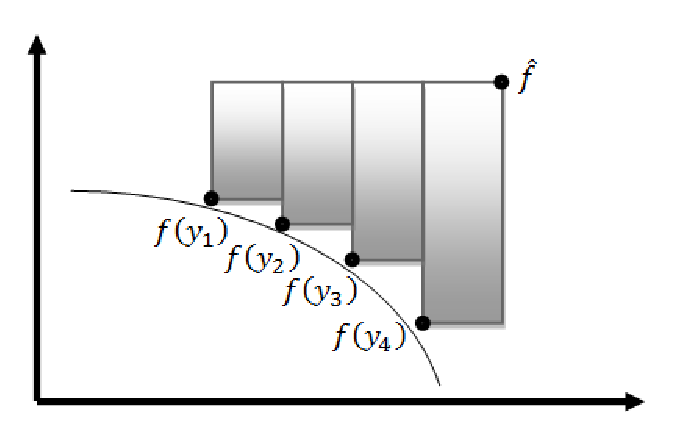
\includegraphics[scale=.5]{fig_01}}
\caption{An example of the hypervolume index (HV) estimate}
\label{fig:01}
\end{figure}

The first benchmark problem is stated as follows \cite{c10}:
\begin{equation}\label{eq:26}
f_1 (y)=(y_1-1) y_2^2+1, f_2 (y)=y_2, 0 \leq y_1,y_2 \leq 1.
\end{equation}

For MAMGS, the following parameters were used: the reliability parameter $r=2$, the accuracy $\epsilon = 0.06$, and 100 subproblems (\ref{eq:06}) have been solved. The reference point was (1,1).\par

The results of the experiments are presented in Table \ref{tab:01}. The column ''Iterations'' shows the total number of the optimization iterations executed by the method (this is the same as the total number of the iteration points at which the objective function values are computed). The column ''PDA points'' demonstrates the number of points included in the numerical approximation of the Pareto domain. The efficiency indicators of the calculated Pareto domain approximations are given in the columns ''HV'' and ''DU''.

\begin{table}[t]
\centering
\caption{Numerical results of the methods compared for the benchmark problem  (\ref{eq:26})}
\label{tab:01}
\begin{tabular}{cllll}
\hline
\textbf{Method} & \textbf{Iterations} & \textbf{PDA points} & \textbf{HV} & \textbf{DU} \\ \hline
MC              & 500                 & 67                  & 0.300       & 1.277       \\
SEMO            & 500                 & 104                 & 0.312       & 1.116       \\
NUC             & 515                 & 29                  & 0.306       & 0.210       \\
BLO             & 498                 & 68                  & 0.308       & 0.175       \\
MAMGS           & 390                 & 90                  & 0.317       & 0.094       \\ \hline
\end{tabular}
\end{table}

To illustrate the obtained results, Figure \ref{fig:01} shows the Pareto domain approximation obtained by using the MAMGS method.

\begin{figure}
\center{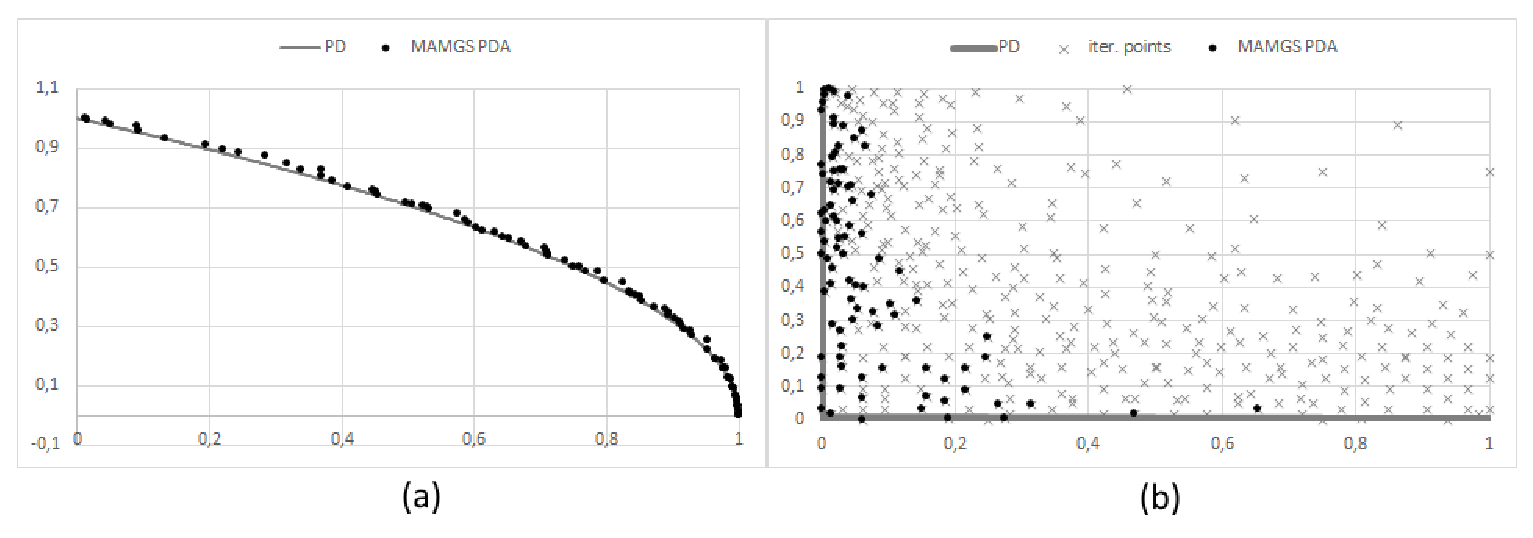
\includegraphics[scale=.4]{fig_02}}
\caption{The Pareto domain approximation (a) and iteration points (b) executed by MAMGS}
\label{fig:02}
\end{figure}

Further, the second benchmark problem has been solved \cite{c10}:
\begin{equation}\label{eq:27}
f_1 (y)=y_1, f_2 (y)=\min {( |y_1-1|,1.5-y_1)}+y_2+1, 0 \leq y_1,y_2 \leq 2.
\end{equation}

For MAMGS, the following parameters were used: the reliability parameter $r=2$, the accuracy $\epsilon = 0.06$, and 100 subproblems (\ref{eq:06}) have been solved. The reference point was (2,3).
The results of the experiments are presented in Table 2 (the values of the DU indicator are not available in \cite{c10,c45}). 

\begin{table}[t]
\centering
\caption{Numerical results of the methods compared for the benchmark problem (\ref{eq:27})}
\label{tab:02}
\begin{tabular}{clll}
\hline
\textbf{Method} & \textbf{Iterations} & \textbf{PDA points} & \textbf{HV} \\ \hline
MC              & 500                 & 22                  & 3.38        \\
SEMO            & 500                 & 221                 & 3.27        \\
NUC             & 490                 & 36                  & 3.42        \\
BLO             & 435                 & 92                  & 3.61        \\
MAMGS           & 380                 & 92                  & 3.59        \\ \hline
\end{tabular}
\end{table}

As shown by the experimental results, MAMGS has an evident advantage over a number of other multicriterial optimization methods, even in solving relatively simple MCO problems.\par

It should be noted that the conditions for this experiment did not correspond to the initial assumptions about the properties of the multicriterial optimization problems: the partial criteria are neither multiextremal nor time-consuming.\par

In the second series of experiments, MAMGS was compared with four other MCO methods considered in \cite{c50}, namely: 
\begin{itemize}
	\item The linear combination method (LCM),
	\item The Multi-Objective Genetic Algorithm (MOGA),
	\item The global criterion method (GCM),
	\item The $\epsilon$-constraint method (ECM).
\end{itemize}
	
The benchmark problems and the numerical results of these methods are taken form \cite{c50}.\par

The first benchmark problem is stated as follows:
\begin{equation}\label{eq:28}
 \begin{cases}
   f_1 (y)=1-\exp \left( -\sum_{i=1}^3{(y_i - 1/ \sqrt{3})^2} \right), \\
   f_2 (y)=1-\exp \left( -\sum_{i=1}^3{(y_i + 1/ \sqrt{3})^2} \right), \\
 \end{cases}
-4 \leq y_1,y_2 \leq 4.
\end{equation}

For MAMGS, the following parameters were used: the reliability parameter $r=1.1$, the accuracy $\epsilon = 0.04$, and 50 subproblems (\ref{eq:06}) have been solved. \par

Because the numerical results in \cite{c50} are given in the graphic form, the results of the experiment are given in the same way -- see Figure \ref{fig:03}. In addition, the number of executed iterations can be indicated: $LCM=258$, $MOGA=2500$, $GCM=286$, $ECM=257$. For MAMGS the number of executed iterations is 283.

\begin{figure}
\center{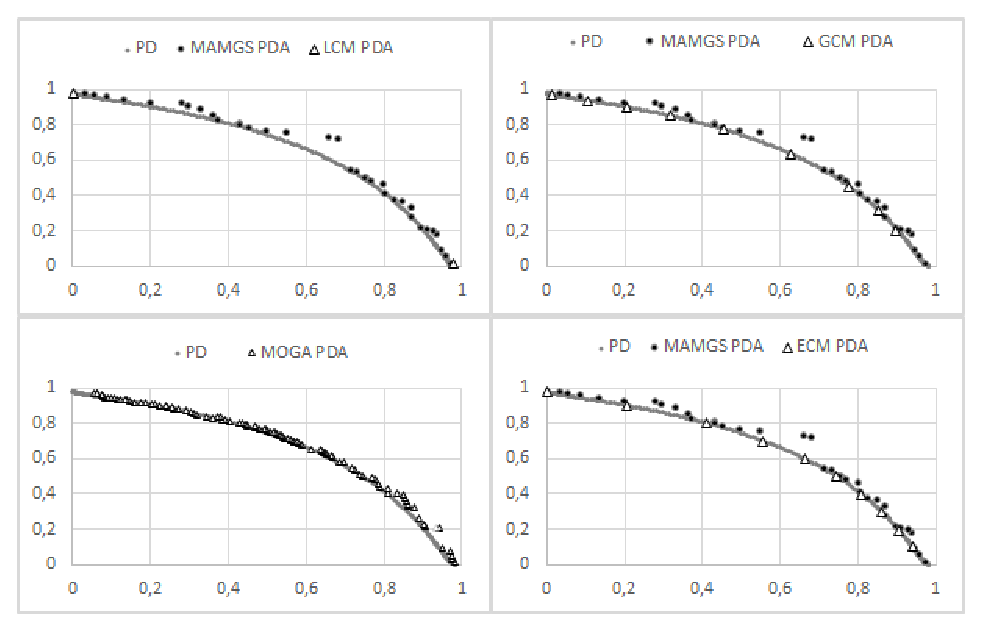
\includegraphics[scale=.5]{fig_03}}
\caption{The Pareto domain approximations calculated by the compared methods for the benchmark problem (\ref{eq:28})}
\label{fig:03}
\end{figure}

The second benchmark problem is stated as follows:
\begin{equation}\label{eq:29}
f_1 (y)=y_1,f_2 (y)=(1+10y_2 ) \left[1-(y_1/(1+ 10 y_2 ))^2-y_1/(1+10y_2 ) sin⁡(8 \pi y_1) \right],
\end{equation}
where $0 \leq y_1,y_2 \leq 1$.\par

For MAMGS, the following parameters were used: the reliability parameter $r=2$, the accuracy $\epsilon = 0.01$, and 50 subproblems (\ref{eq:06}) have been solved.\par

The numerical results are given in the graphic form -- see Figure \ref{fig:04}. In addition the number of executed iterations can be indicated: $LCM=875$, $MOGA=3000$, $GCM=427$, $ECM=575$. For MAMGS the number of executed iterations is 277.

\begin{figure}
\center{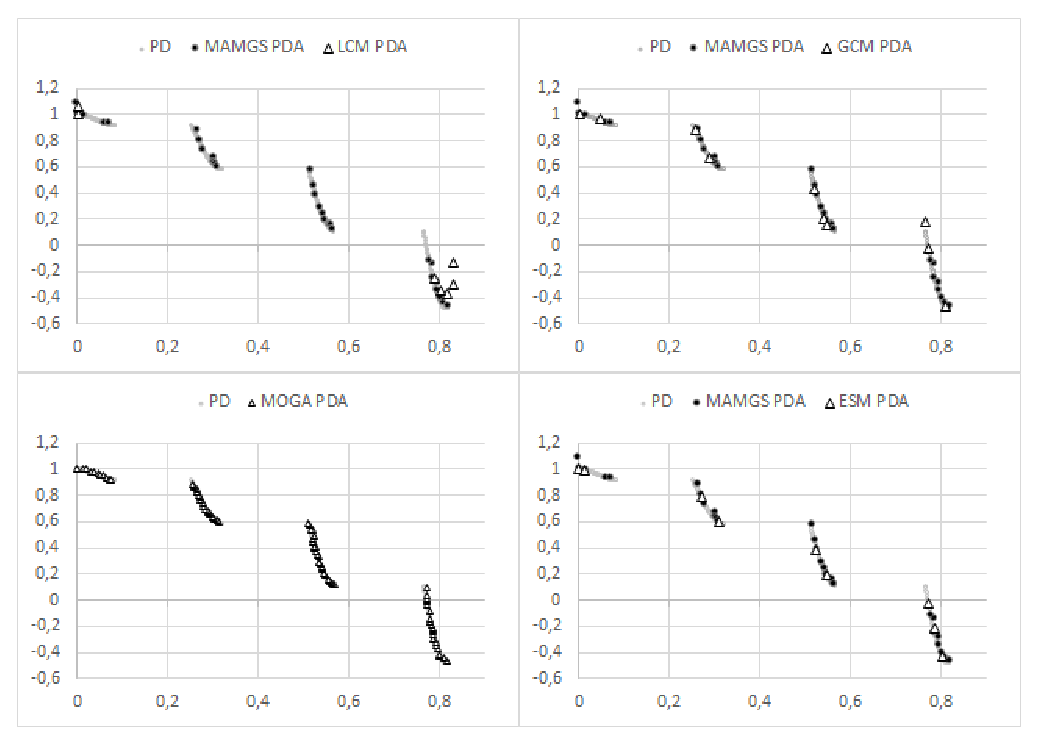
\includegraphics[scale=.5]{fig_04}}
\caption{The Pareto domain approximations calculated by the compared methods for the benchmark problem (\ref{eq:29})}
\label{fig:04}
\end{figure}

In the third series of experiments, the bi-criterial two-dimensional optimization problems have been solved, i.e. $N=2$, $s=2$. To obtain the MCO benchmark problems, the multiextremal functions were generated using the GKLS-generator \cite{c14}. This generator generates the multiextremal optimization problems with a priori known properties: the number of local minima, the size of their attraction domains, the point of global minimum, and the value of the functions therein, etc.\par

For MAMGS the following parameters were used: the reliability parameter $r=4.5$, the accuracy $\epsilon = 0.01$. A total of 100 MCO problems were solved, for each of them 50 global optimization subproblems (\ref{eq:06}) were solved with different convolution coefficients $\lambda$, distributed in $\Lambda$ from (\ref{eq:06}) uniformly. \par
 
The experimental results are shown in Table \ref{tab:03}. The columns ''10'',\dots,''50'' show the average number of optimization iterations executed by the method for solving the indicated set of the subproblems (\ref{eq:06}).

\begin{table}[t]
\centering
\caption{Experimental results for solving two-dimensional bi-criterial problems}
\label{tab:03}
\begin{tabular}{ccccccc}
\hline
Computational results                                                                                  &           & \multicolumn{5}{c}{Number of subprolems being solved}                        \\ \cline{3-7} 
(average per subproblem)                                                                               &           & 10           & 20            & 30            & 40            & 50            \\ \hline
\begin{tabular}[c]{@{}c@{}}Computations without \\ using search information\end{tabular}               &           & 647.7        & 817.8         & 840.6         & 882.0         & 835.2         \\
\begin{tabular}[c]{@{}c@{}}Number of subproblems solved \\ with the required accuracy\end{tabular}     &           & 99.4\%       & 99.1\%        & 98.6\%        & 98.7\%        & 98.8\%        \\
\hline
\begin{tabular}[c]{@{}c@{}}Computations using \\ search information\end{tabular}                       &           & 94.1         & 87.3          & 89.9          & 82.7          & 67.1          \\
\begin{tabular}[c]{@{}c@{}}Number of subproblems solved \\ with the required accuracy\end{tabular}     &           & 99.4\%       & 98.9\%        & 98.6\%        & 98.7\%        & 98.9\%        \\
\hline
\textbf{\begin{tabular}[c]{@{}c@{}}Reduction in the number of \\ optimization iterations\end{tabular}} & \textbf{} & \textbf{6.9} & \textbf{9.4}  & \textbf{9.4}  & \textbf{10.7} & \textbf{12.5} \\ \hline
\end{tabular}
\end{table}

These results show that if the method uses the search information then it can reduce the executed optimization iterations in solving multicriterial optimization problems up to 12.5 times. Moreover, as it has been noted previously, solving each subsequent scalar subproblem (\ref{eq:06}) to find another partial solution of the MCO problem requires a permanently decreasing number of optimization iterations. For  more explicit demonstration of this key property of the proposed approach, Table \ref{tab:04} shows the results of experiments separated by the sequence of solved subproblems (\ref{eq:06}); each group includes 10 scalar subproblems (\ref{eq:05}).

\begin{table}[t]
\centering
\caption{Average number of executed iterations per  a subproblem within successive groups including 10 subproblems}
\label{tab:04}
\begin{tabular}{cccccc}
\hline
\begin{tabular}[c]{@{}c@{}}Number of problems \\ included in a group\end{tabular}                      & 1-10         & 11-20         & 21-30        & 31-40         & 41-50          \\ \hline
\begin{tabular}[c]{@{}c@{}}Computations without \\ using search information\end{tabular}               & 647.7        & 987.8         & 886.2        & 1,006.1       & 648.2          \\
\begin{tabular}[c]{@{}c@{}}Computations using \\ search information\end{tabular}                       & 94.1         & 80.6          & 94.9         & 61.1          & 4.6            \\
\textbf{\begin{tabular}[c]{@{}c@{}}Reduction in the number\\  of optimization iterations\end{tabular}} & \textbf{6.9} & \textbf{12.3} & \textbf{9.3} & \textbf{16.5} & \textbf{139.4} \\ \hline
\end{tabular}
\end{table}

The experimental results presented in Table \ref{tab:04} are even more convincing in showing a significant reduction in computations as the volume of obtained search information increases. Thus, the amount of computations was reduced  139.4 times for the group, which included from 41 to 50 subproblems. \par

For one of the solved problems more complete information is presented in Table \ref{tab:05}. Row 2 contains the characteristics of the Pareto domain approximation computed numerically. In rows 3-4 the results of solving the MCO problem without the reuse of the search information are given for various values of required accuracy of computations. In the last row (row 5), the results of computations with the reuse of the search information are shown. One can see that the best results with respect to the completeness and the uniformity of approximation are presented in row 3 (the computations without the reuse of the search information). However, the number of performed iterations (the computations of the criteria values) exceeds the indicator given in row 5 more than 10 times. At approximately equal allowed number of iterations, the efficiency of computations with the reuse of the search information is higher (see rows 4 and 5). \par

In addition, an experiment on the solving two subproblems with the maximum differing values of the convolution coefficients $\lambda_1=(1,0)$ and $\lambda_2=(0,1)$ has been performed (i. e. the minimizations of the first criterion and of the second one have been performed successively). Total for finding the minimum values of the criteria without the reuse of the search information 855 iterations (the computations of the criteria values) have been executed, whereas with the reuse of the search information 530 iterations were necessary only (for the optimization of the second criterion at $\lambda_2=(0,1)$ 395 iterations have been executed in the former case, and 50 iterations only – in the latter one).\par

\begin{table}[t]
\centering
\caption{The efficiency indicators of the solving of one of subproblems from Experiment 3}
\label{tab:05}
\begin{tabular}{clcclcc}
\hline
\textbf{}                                                                                                  & \textbf{} & \multicolumn{2}{c}{\textbf{Indicators}} & \textbf{} & \textbf{\begin{tabular}[c]{@{}c@{}}Average number \\ of iterations\end{tabular}} & \multirow{2}{*}{\textbf{\begin{tabular}[c]{@{}c@{}}Number of points\\ in PDA\end{tabular}}} \\
\textbf{}                                                                                                  & \textbf{} & \textbf{DU}        & \textbf{HV}        & \textbf{} & \textbf{per subproblems}                                                         &                                                                                             \\ \hline 
Pareto domain approx.                                                                                      &           & 0.039              & 20.852             &           &                                                                                  & 5087                                                                                        \\ \cline{1-1} \cline{3-4} \cline{6-7} 
\begin{tabular}[c]{@{}c@{}}Computations without using \\ search information ($\epsilon=0.01$)\end{tabular} &           & 0.076              & 20.847             &           & 1022.74                                                                          & 803                                                                                         \\ \cline{1-1} \cline{3-4} \cline{6-7} 
\begin{tabular}[c]{@{}c@{}}Computations without using \\ search information ($\epsilon=0.05$)\end{tabular} &           & 0.192              & 20.728             &           & 166.96                                                                           & 123                                                                                         \\ \cline{1-1} \cline{3-4} \cline{6-7} 
\begin{tabular}[c]{@{}c@{}}Computations using \\ search information ($\epsilon=0.01$)\end{tabular}         &           & 0.169              & 20.820             &           & 92.52                                                                            & 200                                                                                         \\ \hline
\end{tabular}
\end{table}

In the fourth experiment, the two-dimensional MCO problem with 5 criteria, i.e. for $N=2$, $s=5$, was solved. The problems were generated using the multiextremal functions generated by the GKLS-generator again. The following values were used: the reliability parameter $r=5$, the search accuracy $\epsilon=0.01$. As in previous experiments, MCO problems (\ref{eq:05}) were solved using 50 different convolution coefficient values. These experiments showed that the average number of optimization iterations for solving a single problem (\ref{eq:06}) without using the accumulated search information was 1,574.7. In the case when the search information was taken into account, the average number of optimization iterations executed by MAMGS was 89.2 (more than a 17-fold reduction).\par

In the final experiment, the bi-criteria five-dimensional MCO problem, i.e. for $N=5$, $s=2$, was solved. The problems were generated using the multiextremal functions generated by the GKLS-generator \cite{c14}. The following values were used: the reliability parameter $r=4$, the accuracy $\epsilon=0.03$. As in the previous experiments, MCO problems (\ref{eq:06}) were solved using 50 different convolution coefficient values. These experiments showed that the average number of optimization iterations for solving a single problem (\ref{eq:06}) without using the accumulated search information was 300,383. In the case the search information was taken into account, the average number of optimization iterations executed by MAMGS was 49,751 (more than 6-fold reduction). 

\section{Conclusion}
The paper proposes an efficient method for solving complex multicriterial optimization problems, for which the optimality criteria can be multiextremal and the calculation of the criteria values can be time-consuming. The proposed approach involves the transformation of multicriterial problems to global optimization problems through the minimax convolution of the partial criteria, the reduction of dimensionality using the Peano curves, and the use of the efficient information-statistical global optimization methods.\par

The key aspect of this approach is related to overcoming the huge computational complexity of the MCO problems. A significant increase in the efficiency and a considerable reduction of the amount of computations are provided by the intensive use of all search information obtained during the process of solving multicriterial optimization problems. As a part of this approach, the methods of recalculating all available search information to the values for the subsequent global optimization problem have been proposed. The updated search information is then used in the global optimization methods for the adaptive selecting of the global search iterations. According to the results of the computational experiments, the proposed approach reduces repeatedly the computational complexity of solving the multicriterial optimization problems.\par

To conclude, it can be noted that the proposed approach is promising and requires further investigation. First of all, it is necessary to continue conducting computational experiments to address the multicriterial optimization problems with a greater number of partial criteria and for greater dimensionality in the optimization problems being solved. The potential for parallel computing should also be evaluated in view of the high computational complexity for solving global optimization problems.

\section*{Acknowledgements}  
This work has been supported by the Russian Science Foundation, project No 16-11-10150 ''Novel efficient methods and software tools for time-consuming decision making problems using superior-performance supercomputers.''




% Non-BibTeX users please use
\begin{thebibliography}{}

\bibitem{c1}	Barkalov, K., Gergel, V.: Parallel global optimization on GPU. Journal of Global Optimization, 1--18 (2015). DOI 10.1007/s10898-016-0411-y.
\bibitem{c2}	Barkalov, K., Gergel, V., Lebedev, I.: Use of Xeon Phi Coprocessor for Solving Global Optimization Problems. LNCS, \textbf{9251}, 307--318. Springer, Heidelberg (2015)
\bibitem{c3}	Barkalov, K., Gergel, V., Lebedev, I.: Solving Global Optimization Problems on GPU Cluster. Simos T.E. (Ed.) ICNAAM 2015, AIP Conference Proceedings, \textbf{1738}, art. no. 400006 (2016)
\bibitem{c4}	Bleuler, S., Laumanns, M., Thiele, L., Zitzler, E.: PISA-A Platform and Programming Language Independent Interface for Search Algorithms. Evolutionary Multi-Criterion Optimization, LNCS, \textbf{2632}, 494--508 (2003)
\bibitem{c5}	Branke, J., Deb, K., Miettinen, K., Slowinski, R. (eds.): Multi-Objective Optimization-Interactive and Evolutionary Approaches. Springer, Berlin (2008)
\bibitem{c6}	Collette, Y., Siarry, P.: Multiobjective Optimization: Principles and Case Studies (Decision Engineering). Springer-Verlag, Berlin, Heidelberg (2011)
\bibitem{c7}	Deb, K.: Multi-Objective Optimization using Evolutionary Algorithms. Wiley, Chichester (2001)
\bibitem{c8}	Ehrgott, M.: Multicriteria Optimization. Springer-Verlag, Berlin, Heidelberg (2005, 2nd ed., 2010)
\bibitem{c9}	Eichfelder, G.: Scalarizations for adaptively solving multi-objective optimization problems. Comput. Optim. Appl., \textbf{44}, 249--273 (2009)
\bibitem{c10}	Evtushenko, Yu.G., Posypkin, M.A.: Method of non-uniform coverages to solve the multicriteria optimization problems with guaranteed accuracy. Automation and Remote Control, \textbf{75}(6), 1025--1040 (2014)
\bibitem{c11}	Figueira, J., Greco, S., Ehrgott, M. (eds.): Multiple criteria decision analysis: State of the art surveys.  Springer, New York (2005)
\bibitem{c12}	Floudas, C.A., Pardalos, M.P.: Recent Advances in Global Optimization. Princeton University Press (2016)
\bibitem{c13}	Gablonsky, J.M., Kelley, C.T.: A Locally-Biased Form of the DIRECT Algorithm. Journal of Global Optimization, \textbf{21}(1), 27--37 (2001)
\bibitem{c14}	Gaviano, M., Lera, D., Kvasov, D.E., Sergeyev, Y.D.: Software for generation of classes of test functions with known local and global minima for global optimization. ACM Trans. Math. Software, \textbf{29}, 469--480 (2003)
\bibitem{c15}	Gergel, V.: A Unified Approach to Use of Coprocessors of Various Types for Solving Global Optimization Problems. 2nd International Conference on Mathematics and Computers in Sciences and in Industry, 13--18 (2015). DOI: 10.1109/MCSI.2015.18 
\bibitem{c16}	Gergel, V., Grishagin, V., Gergel, A.: Adaptive nested optimization scheme for multidimensional global search. J. Glob. Optim., \textbf{66} (1), 35--51 (2016) 
\bibitem{c17}	Gergel, V., Lebedev, I.: Heterogeneous Parallel Computations for Solving Global Optimization Problems. Procedia Computer Science, \textbf{66}, 53--62 (2015). DOI 10.1007/s10898-016-0411-y.
\bibitem{c18}	Gergel, V., Sidorov, S.: A Two-Level Parallel Global Search Algorithm for Solution of Computationally Intensive Multiextremal Optimization Problems. LNCS, \textbf{9251}, 505--515. Springer-Verlag, Berlin, Heidelberg (2015)
\bibitem{c19}	Germeyer, Yu.B.: Introduction in Theory of Operation Research. Moscow, Nauka (1971) (In Russian)
\bibitem{c20}	Grishagin, V.A.: Operating characteristics of some global search algorithms. Problems of Stochastic Search, \textbf{7}, 198--206 (1978) (In Russian)
\bibitem{c21}	Grishagin, V.A., Sergeyev, Y.D., Strongin, R.G.: Parallel characteristic algorithms for solving problems of global optimization. J. Global Optim., \textbf{10}, 185--206 (1997)
\bibitem{c22}	Hill, J.D.: A Search Technique for Multimodal Surfaces. IEEE Transactions on Systems and Cybernetics, \textbf{5}(1), 2--8 (1969)
\bibitem{c23}	Hillermeier, C., Jahn, J.: Multiobjective optimization: survey of methods and industrial applications. Surv. Math. Ind., \textbf{11}, 1--42 (2005)
\bibitem{c24}	Horst, R., Tuy, H.: Global Optimization: Deterministic Approaches. Springer-Verlag, Berlin (1990)
\bibitem{c25}	Kvasov, D.E., Pizzuti, C., Sergeyev, Y.D.: Local tuning and partition strategies for diagonal GO methods. Numerische Mathematik, \textbf{94}(1), 93-106 (2003)
\bibitem{c26}	K{\"o}ksalan, M., Wallenius, J. and Zionts, S.: Multiple criteria decision making: From early history to the 21st century. World Scientific, Singapore (2011)
\bibitem{c27}	Locatelli, M., Schoen, F.: Global Optimization: Theory, Algorithms, and Applications. SIAM (2013)
\bibitem{c28}	Mardani, A., Jusoh, A., Nor, K., Khalifah, Z., Zakwan, N., Valipour, A.: Multiple criteria decision-making techniques and their applications -- a review of the literature from 2000 to 2014. Economic Research-Ekonomska Istra\v{z}ivanja, \textbf{28}(1), 516--571 (2015). DOI: 10.1080/1331677X.2015.1075139
\bibitem{c29}	Marler, R. T., Arora, J. S.: Survey of multi-objective optimization methods for engineering. Struct. Multidisciplinary Optimization, \textbf{26}, 369--395 (2004)
\bibitem{c30}	Miettinen, K.: Nonlinear Multiobjective Optimization. Springer (1999)
\bibitem{c31}	Sergeyev, Y.D., Famularo, D., Pugliese, P.: Index Branch-and-Bound Algorithm for Lipschitz univariate global optimization with multiextremal constraints. Journal of Global Optimization, \textbf{21}(3), 317--341 (2001)
\bibitem{c32}	Sergeyev, Y.D., Grishagin, V.A.: Sequential and parallel algorithms for global optimization. Optimization Methods and Software, \textbf{3}, 111--124 (1994)
\bibitem{c33}	Sergeyev, Y.D., Grishagin, V.A.: Parallel Asynchronous Global Search and the Nested Optimization Scheme. J. Comput. Anal. Appl., \textbf{3}(2), 123--145 (2001)
\bibitem{c34}	Sergeyev, Y.D., Kvasov, D.E.: Global search based on efficient diagonal partitions and a set of Lipschitz constants. SIAM J. on Optimization, \textbf{16}(3), 910--937 (2006)
\bibitem{c35}	Sergeyev, Y.D., Strongin, R.G., Lera, D.: Introduction to global optimization exploiting space-filling curves. Springer-Verlag, New York (2013)
\bibitem{c36}	Siwale, I.: Practical multi-objective programming. Technical Report RD-14-2013. Apex Research Limited (2014)
\bibitem{c37}	Strongin, R.G.: Numerical methods in multiextremal problems: information-statistical algorithms. Nauka, Moscow (1978) (In Russian)
\bibitem{c38}	Strongin, R.G., Sergeyev, Y.D.: Global optimization with non-convex constraints. Sequential and parallel algorithms. Kluwer Academic Publishers, Dordrecht (2000, 2nd ed. 2013, 3rd ed. 2014)
\bibitem{c39}	Pint{\'e}r, J.D.: Global optimization in action (continuous and Lipschitz optimization: algorithms, implementations and applications). Kluwer Academic Publishers, Dortrecht (1996)
\bibitem{c40}	Tan, K.C., Khor, E.F., Lee, T.H.: Multi-objective Evolutionary Algorithms and Applications. Springer-Verlag, London (2005)
\bibitem{c41}	T{\"o}rn, A., {\v Z}ilinskas, A.: Global Optimization. LNCS, \textbf{350}. Springer-Verlag, Berlin (1989)
\bibitem{c42}	Yang, X.-S.: Nature-inspired metaheuristic algorithms. Luniver Press, Frome (2008)
\bibitem{c43}	Zavadskas, E. K., Turskis, Z., Kildien{\.e}, S.: State of art surveys of overviews on MCDM/MADM methods. Technological and Economic Development of Economy, \textbf{20}, 165--179 (2014)
\bibitem{c44}	Zhigljavsky, A.A.: Theory of Global Random Search. Kluwer Academic Publishers, Dordrecht (1991)
\bibitem{c45}	{\v Z}ilinskas, A., {\v Z}ilinskas, J.: Adaptation of a one-step worst-case optimal univariate algorithm of bi-objective Lipschitz optimization to multidimensional problems. Commun Nonlinear Sci Numer Simulat, \textbf{21}, 89--98 (2015)
\bibitem{c46}	Zitzler, E., Knowles, J., Thiele, L.: Quality Assessment of Pareto Set Approximations. LNCS in Multiobjective Optimization-Interactive and Evolutionary Approaches. LNCS, \textbf{5252}, 373--404 (2008)
\bibitem{c47}	Strongin, R.G., Gergel, V.P. Markin, D.L.: Multicriterion multiextreme optimization with nonlinear constraints. Lecture Notes in Economics and Mathematical Systems, \textbf{351}, 120--127 (1988)
\bibitem{c48}	Chinchuluun, A., Pardalos, P.M.: A survey of recent developments in multiobjective optimization. Ann Oper Res, \textbf{154}(1), 29--50 (2007). DOI:10.1007/s10479-007-0186-0
\bibitem{c49}	Pardalos, P.M., {\v Z}ilinskas, A., {\v Z}ilinskas, J.: Non-Convex Multi-Objective Optimization. Springer (2017)
\bibitem{c50}	Chiandussi, G., Codegone, M., Ferrero, S., Varesio, F.E.: Comparison of multi-objective optimization methodologies for engineering applications. Computers and Mathematics with Applications, \textbf{63}(5), 912--942 (2012)
\bibitem{c51}	Zhigljavsky, A., {\v Z}ilinskas, A.: Stochastic Global Optimization. Springer (2008)
\bibitem{c52}	Paulavi{\v c}ius, R., {\v Z}ilinskas, J.: Simplicial Global Optimization. Springer (2014)


\end{thebibliography}

\end{document}
% end of file template.tex
